%%Berichtvorlage für EDBV WS 2015/2016

\documentclass[deutsch]{scrartcl}
\usepackage[ngerman]{babel}
\usepackage[utf8]{inputenc}
\usepackage{algorithmic}
\usepackage{algorithm}
\usepackage{graphicx}
\usepackage{amsmath,amssymb}
\usepackage{subcaption}
\captionsetup{compatibility=false}
\usepackage{multirow}
\usepackage{color}

\begin{document}

\title{Konzept: Projekttitel} %%Projekttitel hier eintragen

\subtitle{EDBV WS 2017/2018: AG\_A2} %%statt XX Arbeitsgruppenbezeichnung hier eintragen (zB.: A1)


%%Namen und Matrikelnummern der Gruppenmitglieder hier eintragen
\author{Jan Michael Lajarno (Matrikelnummer1)\\
Andreas Brunner (Matrikelnummer2)\\
Miran Jank (Matrikelnummer2)\\
Thorsten Korpitsch (01529243)\\
Aleksander Marinkovic (Matrikelnummer2)\\
}



%%------------------------------------------------------

\maketitle


%%------------------------------------------------------

(1-2 Seiten)
\section{Ziel}
Ziel des Projekts\\
\textit{Die gewonnen Schnapskarten werden automatisch erkannt und die Punkte errechnet.}
\section{Eingabe}
Erwarteter Input (.PNG\/.JPG\/.JPEG, Farbbild der Karten)\\
\textit{Der Benutzer muss nur ein Farbbild der Karten (aufgereiht) bereitstellen.}
\section{Ausgabe}
textuell:\\
\textit{Die erreichte Punktzahl wird dem User in Text-Form ausgegeben.}
\section{Voraussetzungen und Bedingungen}
Voraussetzungen für Eingabe definieren, anhand dieser werden Datensätze erstellt\\
\textit{Ein Farbbild der Aufgereihten Karten. Zwischen den Karten muss etwas Platz gelassen werden. Der Hintergrund sollte möglichst Einfarbig sein. Die Kamera soll sich in einem Winkel von 45 bis 90 Grad befinden.}
\section{Methodik}
Methodik- Pipeline
\begin{enumerate}
	\item Geometrische Transformation
	\item Kanten-Filter
	\item Template-Matching
\end{enumerate}
\textit{Kommentar: Die folgenden Fragen sollten hier bedacht und beantwortet werden: Welche Arbeitsschritte sind notwendig um für den gegebenen Input den entsprechenden Output zu berechnen? Wozu sind die jeweiligen Methoden notwendig – d.h. welche konkrete Methoden wird für diese Arbeitsschritte verwendet?}
\section{Evaluierung}
\begin{itemize}
	\item Um das Eingabebild vorzubereiten wird aus dem, bis zu 45 Grad schrägen Bild, ein Bild aus der Vogelperspektive (90 Grad)
	\item Um die einzelnen Spielkarten zu trennen wird eine Kantendetektion durchgeführt.
	\item Um die Spielkarte zu identifizieren wird ein Pattern-Matching durchgeführt.
\end{itemize}
\textit{Kommentar: Eine qualitative Evaluierung basiert auf der subjektiven Wahrnehmung einer Person (Ist ein Ergebnis gut oder schlecht?). Ihr sollte hier aber vor allem auch eine quantitative Evaluierung durchführen, d.h. eine objektive Evaluierung durch Vergleich eurer (Zwischen-)Ergebnisse mit ground truth (ein klassisches Beispiel: Für wie viele der Test-Datensätze wurde für Aufgabe xy ein korrektes Ergebnis erzielt?).}
\section{Datenbeispiel}
\begin{figure}[h!]
 \centering
 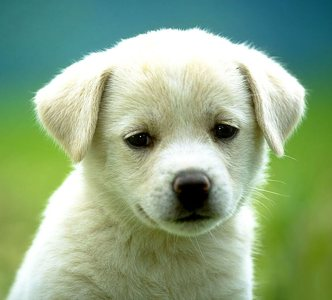
\includegraphics[width=0.4\textwidth]{img.jpg}
 \caption{puppy}
 \label{fig:img}
\end{figure}
\section{Zeitplan}
\begin{table}[h!]
	\centering
		\begin{tabular}{|c|c|c|}
		\hline
		Meilenstein & abgeschlossen am & Arbeitsaufwand in h\\
		\hline
		Projekt aussuchen& 11.10.2017 & 5\\
		Konzept erstellen& ... & ...\\
		... & ... & ... \\
		\hline
		\end{tabular}
\end{table}
\textit{Kommentar: Definiert euch „Meilensteine“. Die vorgegebenen Termine (zB. Zwischenpräsentation) sind hier nicht von Interesse, stellt euch eher die Frage: Wann rechnet ihr mit einem fertigen Prototyp (mit Hilfe von Matlab-Toolboxes)? Wann soll danach ein gewisser Arbeitsschritt (entsprechend eurer Methodik-Pipeline) fertig implementiert sein? Plant auch Zeit für zB. Tests, Evaluierung etc. ein.
Gebt weiters pro Arbeitsschritt an, wieviel Arbeitsaufwand (Stunden) eurer Meinung nach zur Umsetzung notwendig sind. Bedenkt, dass es sich bei EDBV um eine Übung im Ausmaß von 3.0 ECTs handelt. Für 1.0 ECTs rechnet man mit 25h Arbeitsaufwand pro Semester. Auf Teil1 (die Gruppenphase von EDBV) entfallen 2.4 dieser 3.0 ECTs und somit 60h Arbeit pro Gruppenmitglied. Wir rechnen daher für Teil 1 mit 300h Arbeit pro Gruppe.
}\\
\\
\textit{Kommentar: Gebt eine relevante Literaturquelle (Bücher bzw. Kapitel, Konferenz- oder Journal-Papers) pro Gruppenmitglied (im kompilierten Bibtex-Format - Beispiele für Referenzen im Bibtex-Format: http://verbosus.com/bibtex-style-examples.html?lang=de). Diese Quellen sollten für euch bei zB. der Implementierung einer Methode, der Wahl von Parametern, etc. helfen. Können aber auch ein ähnliches Problem behandeln und motivieren, warum ihr euch für gewisse Methodik entschieden habt.}
%%------------------------------------------------------
\bibliographystyle{plain}
\nocite{*}
\bibliography{edbv_lit}
%%Bei verwendung von Latex schreibt ihr eure Referenzen in ein eigenes bib-File (siehe hier Beispiel in edbv_lit.bib). Weitere Information zum Einbinden von BibTex gibt es hier: http://www.bibtex.org/Using/de/
%%------------------------------------------------------

\end{document}
